\section{Results}

This section presents the experimental results of the study, organized according to the two analytical scopes defined in Section~I: (1) the classification performance comparison between ConvNeXt-Tiny and DeiT-Small, and (2) the faithfulness comparison between Grad-CAM and Attention Rollout as measured by deletion and insertion AUC.

\subsection{Hyperparameter Selection}

Both ConvNeXt-Tiny and DeiT-Small were fine-tuned using a two-phase training scheme (linear-probe followed by full fine-tuning) under a grid search over learning rate and number of training epochs. For each architecture, the configuration achieving the highest validation macro-F1 was selected as the final model, following the model selection protocol described in Section~III-A. Table~\ref{tab:hyperparam_selection} summarizes the selected configuration for each architecture.

\begin{table}[htbp]
\caption{Selected Hyperparameter Configuration per Architecture}
\label{tab:hyperparam_selection}
\centering
\begin{tabular}{lcc}
\toprule
\textbf{Hyperparameter} & \textbf{ConvNeXt-Tiny} & \textbf{DeiT-Small} \\
\midrule
Linear probe learning rate & $1\times10^{-3}$ & $1\times10^{-3}$ \\
Full fine-tuning learning rate & $5\times10^{-5}$ & $1\times5^{-5}$ \\
Weight decay & $0.05$ & $0.05$ \\
Label smoothing & $0.1$ & $0.1$ \\
Linear probe epochs & 5 & 5 \\
Full fine-tuning epochs & 45 & 45 \\
Batch size & 32 & 32 \\
\bottomrule
\end{tabular}
\end{table}

The selected configuration for each architecture converged well before its configured epoch budget was exhausted (epoch 11 of 30 for ConvNeXt-Tiny, epoch 19 of 40 for DeiT-Small), consistent with the two-phase fine-tuning scheme reaching its best validation macro-F1 early in the full-fine-tuning phase. The full ranking of all $15$ grid-search combinations per architecture is available in the accompanying evaluation notebook (\texttt{eval.ipynb}).

\subsection{Classification Performance}

Table~\ref{tab:classification_performance} presents the test-set classification performance of both architectures, reported as overall accuracy and macro-averaged precision, recall, and F1-score. Diabetic retinopathy recall is reported separately, as it serves as the tie-breaker criterion for final model selection due to the higher clinical cost of false-negative diagnoses.

\begin{table}[htbp]
\caption{Test-Set Classification Performance}
\label{tab:classification_performance}
\centering
\begin{tabular}{lcc}
\toprule
\textbf{Metric} & \textbf{ConvNeXt-Tiny} & \textbf{DeiT-Small} \\
\midrule
Accuracy & 87.99\% & 87.99\% \\
Macro Precision & 87.91\% & 88.03\% \\
Macro Recall & 87.74\% & 87.77\% \\
Macro F1-score & 87.63\% & \textbf{87.74\%} \\
Macro ROC-AUC & \textbf{98.15\%} & 97.06\% \\
DR Recall (tie-breaker) & \textbf{99.39\%} & 95.76\% \\
\bottomrule
\end{tabular}
\end{table}

Table~\ref{tab:per_class_performance} further reports the per-class precision, recall, and F1-score for the winning model, providing a more detailed view of class-wise classification behavior, particularly for the minority glaucoma class.

\begin{table}[htbp]
\caption{Per-Class Performance of the Selected Model (DeiT-Small)}
\label{tab:per_class_performance}
\centering
\begin{tabular}{lccc}
\toprule
\textbf{Class} & \textbf{Precision} & \textbf{Recall} & \textbf{F1-score} \\
\midrule
Cataract & 93.46\% & 91.67\% & 92.56\% \\
Diabetic Retinopathy & 87.78\% & 95.76\% & 91.59\% \\
Glaucoma & 86.26\% & 74.83\% & 80.14\% \\
Normal & 84.62\% & 88.82\% & 86.67\% \\
\bottomrule
\end{tabular}
\end{table}

Based on the test-set macro-F1, DeiT-Small (87.74\%) marginally outperformed ConvNeXt-Tiny (87.63\%) -- a gap of only $0.11$ percentage points, small enough that the two architectures are effectively comparable in overall discriminative power. Since the macro-F1 values were not exactly tied, the diabetic retinopathy recall tie-breaker was not formally invoked; however, it is worth noting that ConvNeXt-Tiny attained a substantially higher DR recall ($99.39\%$ vs. $95.76\%$) and macro ROC-AUC ($98.15\%$ vs. $97.06\%$), a discrepancy discussed further in Section~IV-E. Per the strict macro-F1 ranking, DeiT-Small is treated as the best-performing architecture and is used as the subject of the per-class analysis above; both architectures' checkpoints are nonetheless carried forward into the explainability analysis in the following subsections, since faithfulness is compared architecture-to-architecture (Grad-CAM vs. Attention Rollout) rather than reduced to a single winner. Both models show the same qualitative weak point: glaucoma has the lowest recall of the four classes ($74.83\%$ for DeiT-Small), reflecting its status as the dataset's minority class (Table~\ref{tab:dataset}).

Fig.~\ref{fig:confusion_matrix} shows the row-normalized confusion matrix of the selected model (DeiT-Small) on the test set, confirming that glaucoma is most frequently confused with cataract and normal, while diabetic retinopathy and cataract are both classified with high recall.

\begin{figure}[htbp]
    \centering
    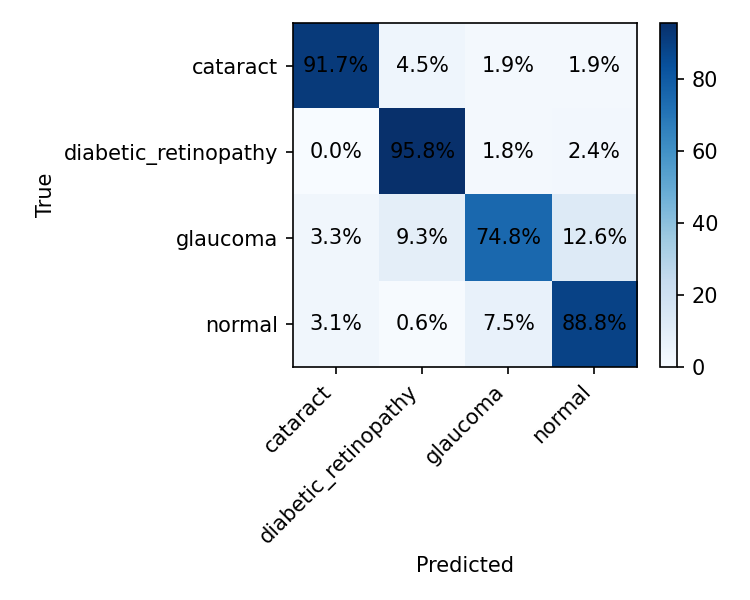
\includegraphics[width=0.45\textwidth]{figures/confusion_matrix.png}
    \caption{Normalized confusion matrix of the selected model (DeiT-Small) on the test set.}
    \label{fig:confusion_matrix}
\end{figure}

\subsection{Qualitative Explainability Results}

Fig.~\ref{fig:xai_qualitative} presents qualitative examples of Grad-CAM heatmaps generated from ConvNeXt-Tiny and Attention Rollout heatmaps generated from DeiT-Small on representative test images from each class. For glaucoma and diabetic retinopathy, both methods concentrate their highest activations tightly on the optic disc region -- the clinically relevant structure for assessing cupping in glaucoma and a common site of hemorrhages and exudates in diabetic retinopathy -- indicating that both models learned to attend to anatomically meaningful evidence rather than spurious background cues for these two classes. For the normal example, both methods likewise center on the optic disc and surrounding vasculature, consistent with this being the reference structure clinicians inspect first. Cataract is the weakest case for both methods: Grad-CAM activates a narrow vertical strip near the image border rather than a diffuse haze pattern (the actual visual signature of a cataract in a fundus photo), while Attention Rollout spreads its attention toward the image corners and edges outside the fundus circle. This is consistent with cataract's presentation as a global loss of image sharpness/contrast rather than a spatially localized lesion, which is inherently harder for patch-level saliency methods -- both CNN- and attention-based -- to localize. Attention Rollout's tendency to assign non-trivial weight to border/corner patches across multiple classes also matches its characterization in Section~III-B as producing more diffuse heatmaps than Grad-CAM.

\begin{figure*}[t]
    \centering
    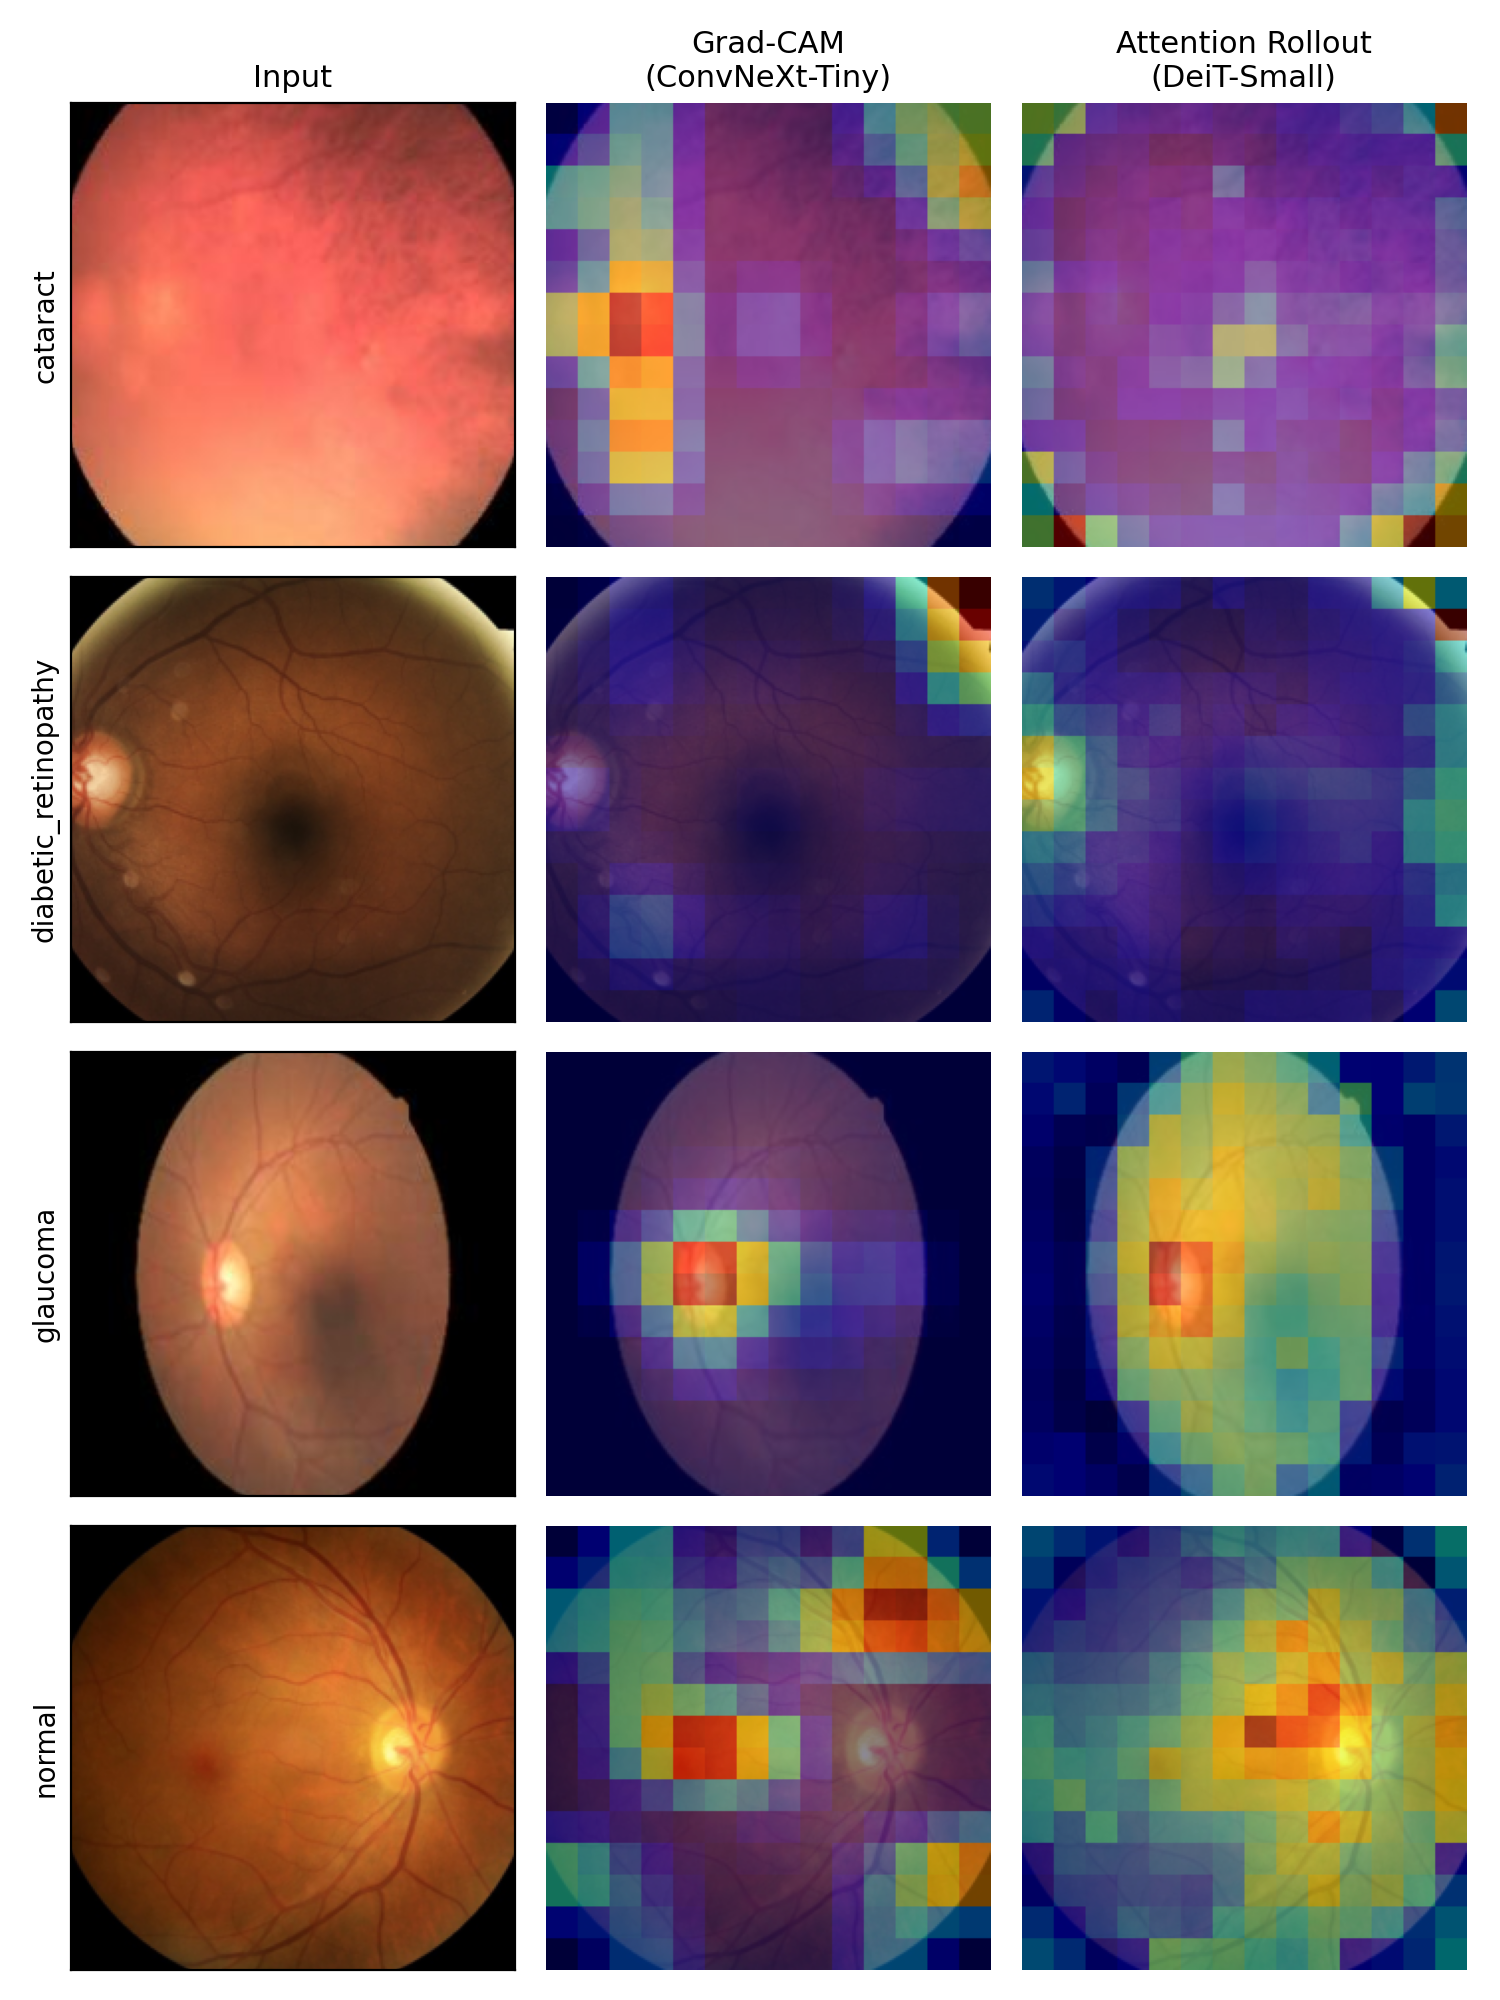
\includegraphics[width=\textwidth,height=0.85\textheight,keepaspectratio]{figures/xai_qualitative_comparison.png}
    \caption{Qualitative comparison of Grad-CAM (ConvNeXt-Tiny) and Attention Rollout (DeiT-Small) heatmaps across the four eye disease classes.}
    \label{fig:xai_qualitative}
\end{figure*}

\subsection{Faithfulness Evaluation}

To quantitatively assess the faithfulness of the generated explanations, deletion and insertion AUC were computed for Grad-CAM on ConvNeXt-Tiny and Attention Rollout on DeiT-Small using patch-based perturbation, as described in Section~III-C. Table~\ref{tab:faithfulness} summarizes the resulting scores, averaged across the test set.

\begin{table}[htbp]
\caption{Deletion and Insertion AUC of Grad-CAM and Attention Rollout ($n=40$ sampled test images)}
\label{tab:faithfulness}
\centering
\begin{tabular}{lcc}
\toprule
\textbf{XAI Method} & \textbf{Deletion AUC} $\downarrow$ & \textbf{Insertion AUC} $\uparrow$ \\
\midrule
Grad-CAM (ConvNeXt-Tiny) & \textbf{0.3906} & 0.6982 \\
Attention Rollout (DeiT-Small) & 0.4626 & \textbf{0.7263} \\
\bottomrule
\end{tabular}
\end{table}

A lower deletion AUC indicates that the regions identified as important are indeed critical to the model's prediction, whereas a higher insertion AUC indicates that the highlighted regions are sufficient to recover the model's confidence. The two methods split the faithfulness comparison: Grad-CAM is more faithful under deletion (confidence collapses faster once its tightly localized high-activation regions are removed), while Attention Rollout is more faithful under insertion (its more diffuse attention pattern is more effective at partially recovering confidence once even a modest fraction of highlighted patches is revealed). This is consistent with the qualitative pattern in Fig.~\ref{fig:xai_qualitative}: Grad-CAM's sharper, more concentrated activations make it more brittle when its narrow high-activation region does not fall on the pathology (as in the cataract example), whereas Attention Rollout's broader coverage is less precise but more robust to partial evidence. Per-class breakdown (available in \texttt{eval.ipynb}) shows both methods are most faithful on glaucoma (deletion AUC of $0.14$ for Grad-CAM and $0.09$ for Attention Rollout), where the pathology is concentrated at a single, well-localized structure (the optic disc), and least faithful on cataract, matching the qualitative finding that neither method localizes cataract's diffuse presentation well.

\subsection{Discussion}

Taken together, the classification and explainability results indicate that overall predictive accuracy and explanation faithfulness are not the same axis of comparison, and neither architecture dominates on both. DeiT-Small edges out ConvNeXt-Tiny on test macro-F1 by a negligible margin ($87.74\%$ vs. $87.63\%$), while ConvNeXt-Tiny is clearly preferable on diabetic retinopathy recall ($99.39\%$ vs. $95.76\%$) and macro ROC-AUC ($98.15\%$ vs. $97.06\%$) -- and its paired explanation method, Grad-CAM, is also the more faithful of the two under deletion. For a clinical screening system where missing a diabetic retinopathy case is the costlier error and clinicians need tightly localized visual evidence to trust a prediction, ConvNeXt-Tiny with Grad-CAM is the more defensible choice despite its very slightly lower macro-F1. Conversely, DeiT-Small with Attention Rollout attains marginally higher overall macro-F1 and a higher insertion AUC, which may suit contexts that value broader contextual corroboration over pinpoint localization. This reinforces the motivation stated in Section~I: accuracy comparison alone is insufficient for selecting a deployable architecture, and faithfulness metrics surface trade-offs that accuracy hides.

This study has several limitations. The hyperparameter search covered only $3$ learning rates $\times$ $5$ epoch budgets ($15$ configurations) per architecture, so the reported results reflect the best configuration found within this grid rather than a globally optimal one. Faithfulness scores were computed on a $40$-image subsample of the test set per architecture rather than the full test set, for computational tractability; the resulting deletion/insertion AUC values should be read as estimates. The qualitative comparison in Fig.~\ref{fig:xai_qualitative} is illustrative (one image per class) rather than an exhaustive audit, and a larger-scale clinical validation with ophthalmologist-annotated lesion masks would be needed to more rigorously confirm the anatomical relevance of the highlighted regions. Finally, both models were fine-tuned and evaluated on a single dataset of $4{,}217$ images from one source; generalization to other fundus imaging devices, populations, or class distributions remains untested.
